\documentclass[10pt]{article}
\usepackage[utf8]{inputenc}
\usepackage[activeacute,spanish]{babel}
\usepackage{amsmath}
\usepackage{amsfonts}
\usepackage{enumerate}
\usepackage{float}
\usepackage{indentfirst}
\usepackage{graphicx}
\usepackage{url}
\usepackage{multicol}
\usepackage{subfigure}
\usepackage[position=bottom]{subfig}
\usepackage[legalpaper, margin=1cm]{geometry}
% \usepackage{fullpage}
\usepackage{algorithm}
\usepackage{algorithmic}
\usepackage{caption}
% \usepackage[caption=false]{subfig}
% \setlength\parindent{0pt}
\usepackage{nopageno}

\usepackage{fancybox}
\usepackage{amsmath, amsfonts, amssymb}

\usepackage{tikzit}
\input{styles.tikzstyles}




\begin{document}

\thispagestyle{empty}

\begin{minipage}[t]{0.6\textwidth}

{\LARGE \textbf{INF152} Estructuras Discretas}

{\large Profesores: R. Astudillo -- M. Bugueño}

Universidad Técnica Federico Santa María

Departamento de Informática -- Diciembre 11, 2020.

\end{minipage}
\hfill
\begin{minipage}[t]{0.35\textwidth}
%RELLENE CON SUS DATOS PERSONALES:
\textbf{Nombre}: Maximiliano Sepúlveda\\[0.3cm]
  \textbf{Paralelo}: 200
\end{minipage}

\vspace{0.8cm}

{\Large Certamen 3 -- Pregunta 2}

\vspace{0.4cm}

\textbf{Esta evaluación tiene como máximo 30 puntos del C3}.

\noindent Para evitar la transmisión del covid-19 entre los funcionarios de la salud se pide como requisito que toda habitación cerrada de un hospital
tenga presión negativa, evitando así la transmisión aérea del virus. Hacer retrofit de presión negativa a hospitales que ya fueron construidos toma mucho tiempo, por lo que un ingeniero propuso que para cada área del hospital deberá existir una fuente y un sumidero encargados de distribuir el aire. El área que estudiaremos tiene los siguientes tubos de ventilación con las capacidades declaradas en los arcos.
\begin{center}
  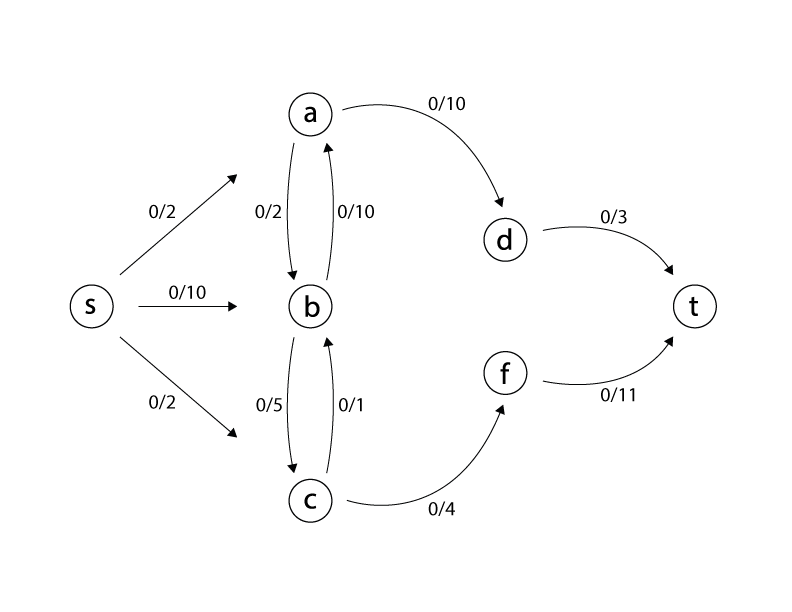
\includegraphics[scale=0.5]{BASE.png}
\end{center}

\begin{enumerate}[1)]
\item Proponga un flujo para esta red que sea máximo. Para esto debe mostrar los \emph{augmenting path} \textbf{[12 puntos]} y una prueba de maximalidad \textbf{[8 puntos]}.

% INDIQUE ACA SU RESPUESTA
\rule{5cm}{0.4pt}

\underline{\textbf{Respuesta:}}

Desde el flujo inicial, se puede armar una red residual (en azul se representa la dirección original del flujo):
\ctikzfig{residual1}
Ahora podemos elegir un \textit{augmenting path} para aumentar el flujo, en este caso, se usará el siguiente:
\[\boxed{s \rightarrow b \rightarrow c \rightarrow f \rightarrow t \qquad (4)}\]

\newpage

Una vez hecho el aumento (de 4), la red de flujo y la red residual quedan de la siguiente forma:
\ctikzfig{flujo2}
\ctikzfig{residual2}
Un siguiente \textit{augmenting path} puede ser el siguiente:
\[\boxed{s \rightarrow b \rightarrow a \rightarrow d \rightarrow t \qquad (3)}\]
Quedando así la siguiente red de flujo y red residual:
\ctikzfig{flujo3}
\ctikzfig{residual3}
Podemos notar que ahora mismo ya no hay ningún \textit{augmenting path} disponible. Podemos fijarnos ahora en la red de flujo y ver donde puede existir un corte.
\ctikzfig{flujo4}
Para poder demostrar que este es un flujo máximo, se debe encontrar un corte; para esto, se definirán los conjuntos $S=\{s,a,b,c,d\}$ y $T=\{f,t\}$., y mediante el teorema Max-Flow Min-Cut se tiene que:
\ctikzfig{corte}
\[\shadowbox{\(\displaystyle \text{Por lo tanto, segun el teorema Max-Flow Min-Cut, el flujo maximo de la red es de 7.} \)} \blacksquare\]


\rule{5cm}{0.4pt}











\item Debido a la alta demanda, es necesario modificar la red de distribución pero, por un tema de presupuesto, solo se puede agregar un único arco \((f,d),(d,f),(c,d)\). Considerando que entre más capacidad tenga el arco más costoso será, elija una de las tuberías (de los arcos anteriores) para agregar al sistema indicando su capacidad de modo tal que se maximice el flujo y se minimice el costo. Justifique su respuesta entregando una prueba de ello \textbf{[10 puntos]}.


% INDIQUE ACA SU RESPUESTA
\rule{5cm}{0.4pt}

\underline{\textbf{Respuesta:}}

Se requiere crear una nueva tubería, pero solo se puede elegir uno de los 3 que se presentan. Si la idea es elegir uno de tal forma que el flujo máximo aumente mas de lo que estaba, y gastando lo mínimo; en este caso, seria ideal que al poner la nueva tubería, el flujo máximo no se vea disminuido o que se quede igual.

Considerando el flujo máximo que se consiguió en el ejercicio anterior, se puede concluir a simple vista que las tuberías $(c,d)$ y $(f,d)$ no van a mejorar el flujo.
\ctikzfig{flujo5}

\newpage

Las tuberías $(c,d)$ y $(f,d)$ no añaden nuevos \textit{augmenting paths}, por lo tanto, no puede mejorar el flujo más de lo que esta. En cambio La tubería $(d,f)$ si puede añadir un nuevo \textit{augmenting path}, mas aun, la tubería $(d,f)$ puede tener una capacidad de hasta 6 unidades antes de que las tuberías $(s,a)$, $(s,b)$ y $(s,c)$ lleguen a su máxima capacidad.

Los \textit{augmenting paths} en cuestión serian los siguientes:
\[s \rightarrow b \rightarrow a \rightarrow d \rightarrow f \rightarrow t \qquad (3)\]
\[s \rightarrow a \rightarrow d \rightarrow f \rightarrow t \qquad (2)\]
\[s \rightarrow c \rightarrow b \rightarrow a \rightarrow d \rightarrow f \rightarrow t \qquad (1)\]

\ctikzfig{flujo6}

Para maximizar el flujo, lo ideal seria poner una tubería en $(d,f)$ con capacidad de 6, aunque con capacidad 1 de igual forma aumentaría el flujo máximo.

\rule{5cm}{0.4pt}

Demostración:

\ctikzfig{camb1}
\[s \rightarrow b \rightarrow a \rightarrow d \rightarrow f \rightarrow t \qquad (3)\]
\ctikzfig{camb2}
\[s \rightarrow a \rightarrow d \rightarrow f \rightarrow t \qquad (2)\]
\ctikzfig{camb3}
\[s \rightarrow c \rightarrow b \rightarrow a \rightarrow d \rightarrow f \rightarrow t \qquad (1)\]
\ctikzfig{camb4}

\ctikzfig{corte2}
\hfill \(\blacksquare\)



\end{enumerate}

%RECUERDE PONER NOMBRE, ROL Y PARALELO EN EL ENCABEZADO
\end{document}
